\documentclass[12pt]{article}
\usepackage{wkrpt}
\begin{document}


\title{Backing Database System for a Messaging Platform Startup}
{
	Ten Thousand Coffees\\
	Toronto, ON
}
{
	Clement Hoang\\
	2B Software Engineering\\
	20531116\\
	c8hoang\\
	May 4th, 2015
}


\letter{Backing Database System for a Messaging Platform Startup}{2A}{Ten Thousand Coffees}{Software Engineering}
{
	\noindent
	Clement Hoang\\
	333 King Street North\\
	Waterloo, ON. 2Z1 N2J
}
{
	Ten Thousand Coffees is startup whose main product is a social networking platform directed towards connecting students with industry professionals. Employed as a member of the core development team for Ten Thousand Coffees, I worked on improving the site and starting experiments over the course of the term. One of the tasks that I was entrusted with was the addition of messaging functionality to Ten Thousand Coffee's online platform.
}
{
	From the the initial planning phase of the messaging system until now, there were several changes of requirements, as well as a limited budget for development. One of the fundamental decisions to make during planning phase was the database system to utilizes for this project. This report analyzes two database systems suitable for backing the messaging platform, and identifies the more appropriate alternative for the project.
}
{
	I would like to thank my co-workers at Ten Thousand Coffees for their continuous guidance during my stay with them. Additionally, I would like to especially thank Elliott Garcea, the lead engineer at Ten Thousand Coffees, for his detailed discussion about our platform's design decisions with me. Finally, I would like to thank my friend, Raymond Wan, for answering a lot of questions that I have about relational database management systems.
}
{
	Clement Hoang, 20531116
}


\tocsection{Executive Summary}
blah blah
The Executive Summary is a one-page summary of the report's highlights, including the purpose and scope of the report, the major points in the report, highlights of the conclusions, and highlights of the recommendations. It is self contained, and is meant to be read and understood by someone (e.g., a company executive officer) who is not likely to read the report itself.

- something about startups
- something about mysql and mongodb (background about traditional relational vs non-relational debate, hard to decide without ocntext, both solve different use cases)
- something about how message is modelled

\newpage


\toc
\lof
\lot


\pagenumbering{arabic}
\section{Introduction}
For several decades, the amount of technological startups has been growing and exploring a vast amount of business models to meet the needs of an ever-changing market. From dating sites to smart-watches, there is a business for almost every idea imaginable. Upon closer inspection of the aforementioned startups, there are noticeably many web applications which are primarily focused on messaging, or, at the very least, include a messaging component. To enable messaging capabilities in a web application, there needs to be a web-server to act as the communication bridge between different users, a database to persist user and message data onto for later usage, and a user interface to allow different people to interact with the web application and message other users. The database, in particular, is very important because it serves as a central store for writing and retrieving user generated content such as message content, chat history logs, and various other datasets for use by the application; without the database, a messaging application simply ceases to function.

However, this is where the startup aspect of Ten Thousand Coffees comes into play. Ten Thousand Coffees is a web application that enables users on the site to connect with one another and invite other parties for coffee chats. As a growing company striving to survive in a fierce environment, the importance of a flexible, scalable, and affordable solution is paramount. This is because startups are limited in budget, and have the need the for high growth. In order to have be successful, a startup must be efficient in using the resources that it can afford, and make decisions that enable them to scale both quickly, and affordably, so that they could outperform the competition. For the Ten Thousand Coffees platform, many technical decisions were made during the planning phase, and one such decision was to use MongoDB, a new, open-sourced NOSQL database that is based on a document object model that features horizontal scalability as well as a dynamic schema that allows for agile development. MongoDB was chosen over a traditional SQL database such as MySQL. In contrast, SQL databases have been around for much longer than NOSQL databases, and therefore have gained a lot of enterprise users. A SQL database such as MySQL and a NOSQL database such as MongoDB have completely different design principles, and this report will explore why Ten Thousand Coffees chose MongoDB over MySQL.

\section{Background}
As mentioned in the introduction earlier, Ten Thousand Coffees is a social platform whose mission is to connect the youth of today with the leaders of tomorrow over coffee chats. The solution that the company decided on to approach this problem was a web platform that allows the discovery of possible coffee candidates, with a messaging and scheduling system that allows users to first chat online, before setting up a meeting via the platform and meeting up in real life. The team consists of a business team and a development team, of which contain five and seven employees correspondingly. As a startup with a small team and therefore, limited manpower, there were certain requirements that the chosen database would have to meet in order to be feasible for the platform. These requirements include the ability to prototype rapidly, to be able to scale well, and to be easy-to-use, while still meeting the performance standards for a modern web application. In order to meet these requirements, the team unanimously decided on the MEAN stack, which is a fullstack Javascript framework that became popular over the past few years. For more information on how a web application architectured with the MEAN stack works, see Appendix A.


\section{Schema Flexibility}

The ability to prototype rapidly is critical to a startup because at the early stages of a company, there is no absolute path from beginning to end goal. This means that the requirements will continuously change and adapt based on feedback received from consumers as well as data gathered by analytics. Because of the need to be able to iterate and improve the platform quickly based on changing requirements, the database management system that is used will need to be flexible so that data can quickly and easily be migrated to support the changing requirements. In this section, the abilities of MongoDB and MySQL to meet the requirements of fast prototyping through schema flexibility will be explored.

The criterion of ``schema flexibility'' refers to the ability of a database to adapt to the changing of the data schema. This is an important measure when comparing the benefits of each database system for a messaging platform startup because through the lifetime of the application, the requirements will continuously evolve to meet the demands of the consumers, and it is also not uncommon for bugs at the schema design level to be introduced where a database schema change is necessary in order to fix it.

For example, an early prototype of a messaging platform may only support conversations in which one user can message only one other user. Obviously, most dedicated messaging platforms will eventually improve its functionality to support features such as multi-user messaging, but as an early iteration, to be able to message only one other user is sufficient. Another scenario in which a schema change may be necessary is when a boolean flag field needs to be added into the schema to contain additional state knowledge will helps to solve certain bugs. In these cases, the database management system that is used should be able to migrate or adapt data from the schema of an earlier iteration with a schema of a later iteration with relative ease in order to be a good fit for a startup.

\subsection{MongoDB}
MongoDB is a NOSQL database that differs from a MySQL database in that it uses dynamic schemas. Consequently, the documents stored in a collection do not need to have a uniform data model. This schema flexibility allows for migration methods that are different from the usual script method, in which a large script is executed against the database to modify the data models all the relevant data stored in the database at once. With MongoDB's dynamic schema, an alternative approach to schema migration, known as ``lazy updating'' or ``schema versioning.'' Lazy updating refers to the method of only updating documents as required, having code that supports both the older schema as well as the newer one. This allows the database to slowly migrate without any downtime or a large change all at once, until the older schema version is eventually deprecated and support is dropped. At Ten Thousand Coffees, I led the migration of the older messaging schema into the new architecture in order to add support for group messaging. For the sake of brevity, the details of the migration are ommitted from this section. See appendix B for the case study.

\begin{figure}
\begin{center}
        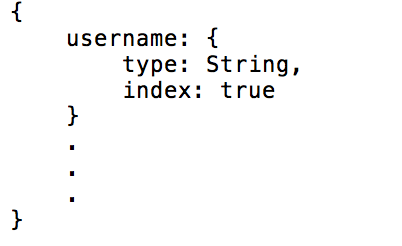
\includegraphics[scale=0.8]{resources/user_schema.png}
\end{center}
\caption{\label{figcaption} A MongoDB user schema for supports group messaging}
\end{figure}

\begin{figure}
\begin{center}
        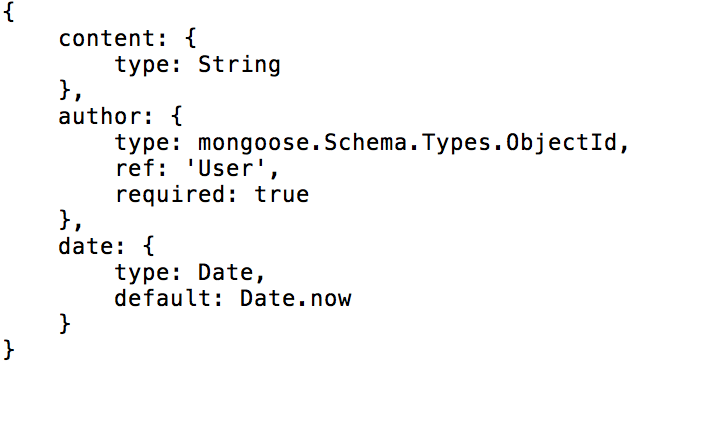
\includegraphics[scale=0.8]{resources/message_schema.png}
\end{center}
\caption{\label{figcaption} A MongoDB message schema for supports group messaging}
\end{figure}

\begin{figure}
\begin{center}
        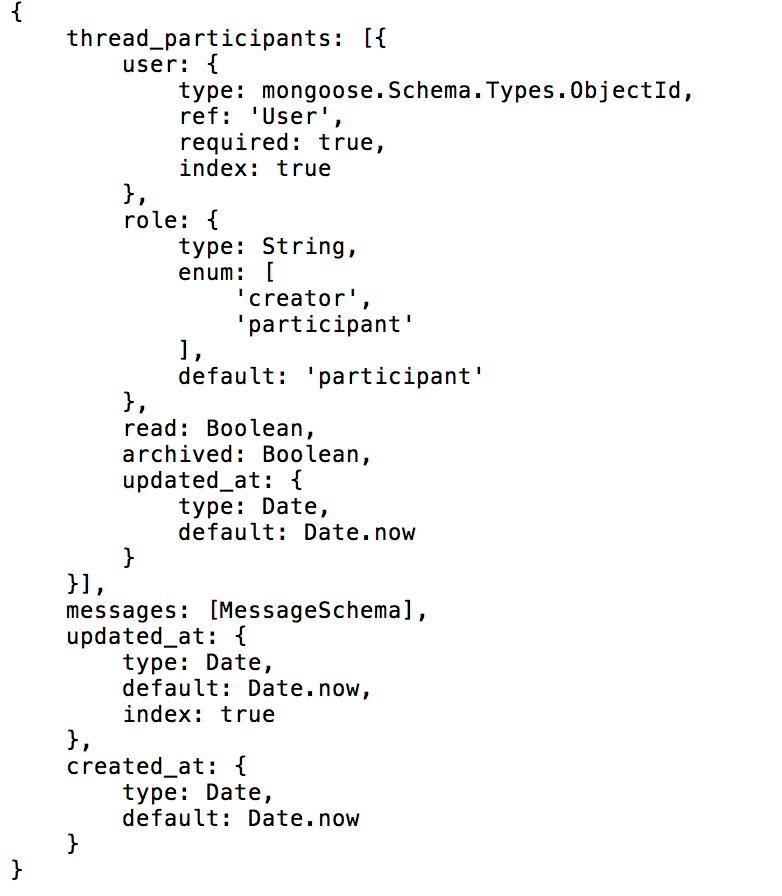
\includegraphics[scale=0.8]{resources/thread_schema.png}
\end{center}
\caption{\label{figcaption} A MongoDB thread schema for supports group messaging}
\end{figure}

\subsection{MySQL}
MySQL is a SQL-compliant database which forces the user to define a structure in terms of tables and columns before data can be stored in it. As such, it demands a long initial setup time. This rigidness comes with benefits such as being more reliable and being more efficient at complex queries \cite{sql_vs_nosql}. However, while these benefits are great for a more corporate enterprise solution such as banking software, where reliability is more important, they are not as suited for a startup that is focused on a messaging platform. By SQL's nature, it is more complex to set up then MongoDB, and migrations would also require significantly more effort, as the the mathematical structure containing tables and rows would require a more revamping than simplying adding/removing a field in the case of MongoDB. This is not good for a company that needs fast prototyping. The advantages of rapid prototyping far outweigh the advantages of transaction safety in a startup, and moreso in a messaging platform. In the worst case, if MongoDB performance is bad on certain queries, the relevant components can be swapped for something that is more performant such as Redis. Therefore, MongoDB is more suitable than MySQL is terms of schema flexibility.

\begin{figure}
\begin{center}
        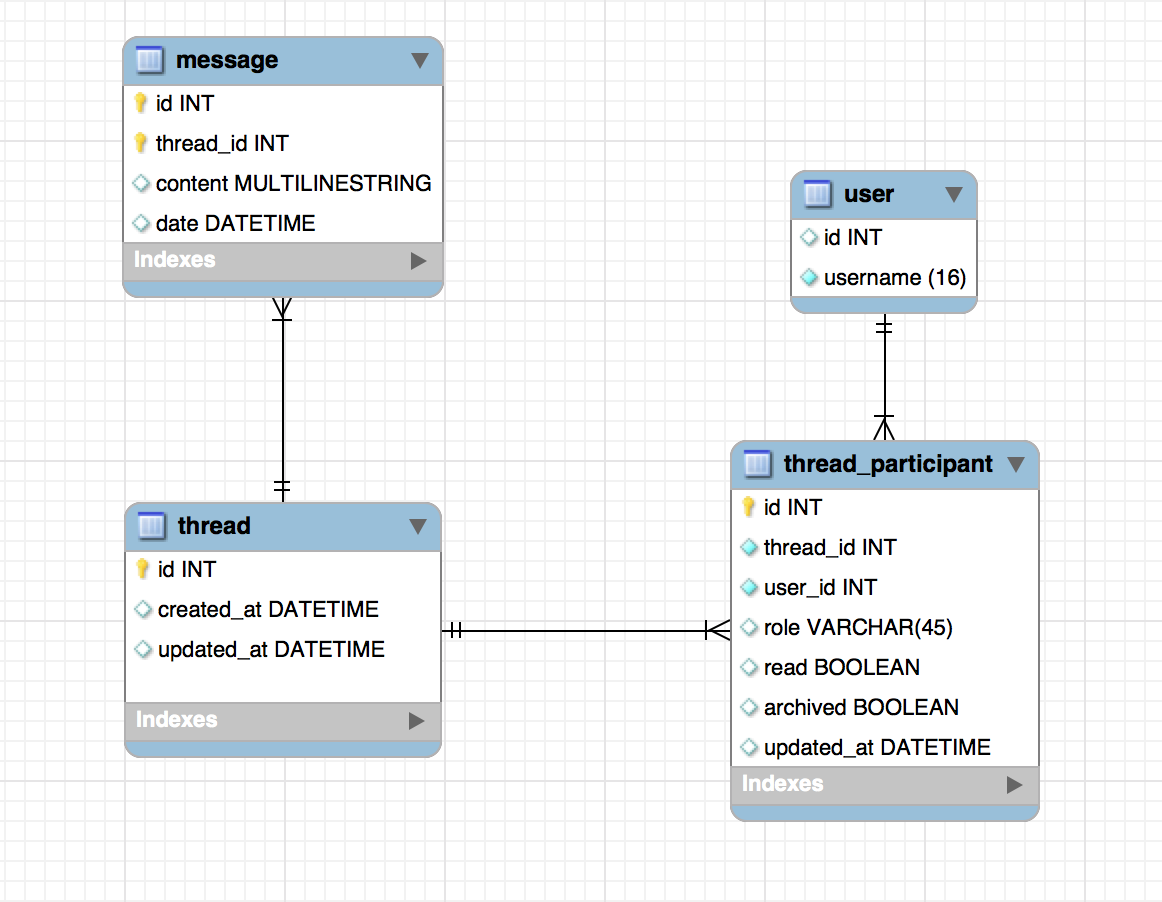
\includegraphics[scale=0.8]{resources/mysql_schema.png}
\end{center}
\caption{\label{figcaption} A MySQL schema that supports group messaging \cite{cap_picture}}
\end{figure}

\section{Scaling}

In a startup, the ability for a database to scale is very important. As a startup often starts off with a limited budget and a small initial consumer base, their product does not need to support high traffic. However, as the company grows and their amount of users rises, then the ability to support the increased traffic is mandatory in order for the company to survive. Different technologies have different techniques to handle specific use cases and so, the characteristics of different databases will vary when they scale. There is a common theorem known as the ``CAP'' theorem where no system can achieve consistency, high-availability, and partition-tolerance at the same time, and this is made especially apparent when scaling the database management system. A consistent system is one where the system can guarantee that the same state will be reported at all nodes in every subsequent operation until the state is explicitly changed. A system that is highly available is one that is resistant to hardware failure and allows operations to continue even if a node has failed. Finally, a partition-tolerant system is one where the system can be split over several datacenters while staying synchronized with one another. \cite{cap_theorem} For a messaging platform, high availability and partition-tolerance is valued more than consistency.

\begin{figure}
\begin{center}
        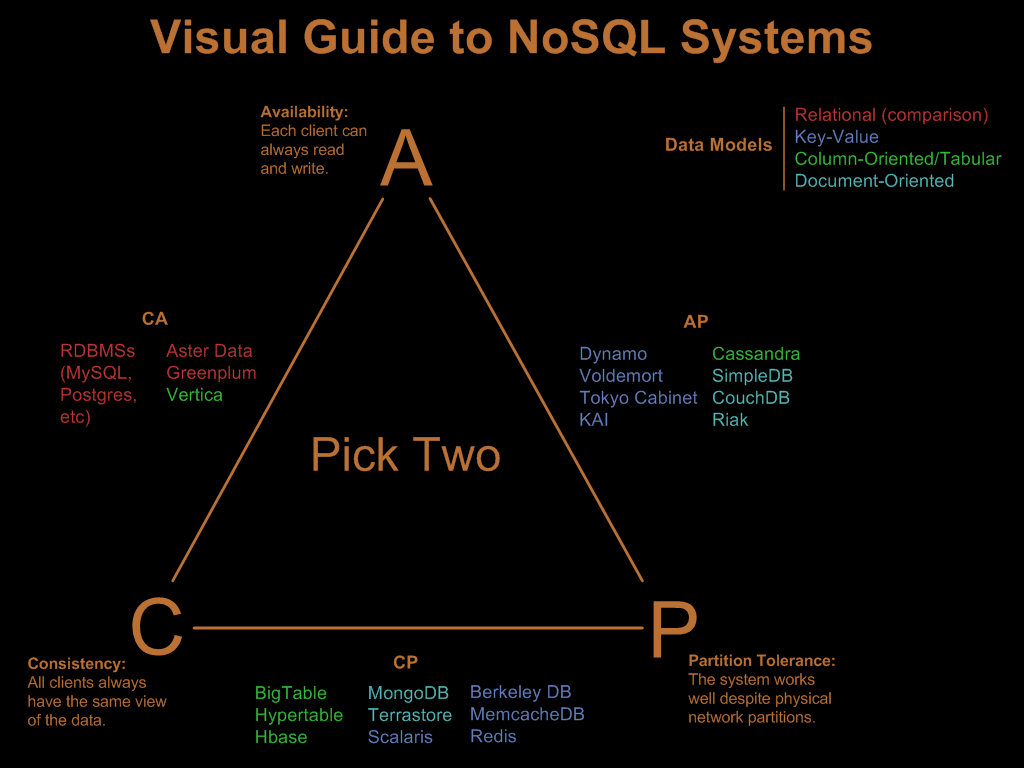
\includegraphics[scale=0.4]{resources/choose_two.png}
\end{center}
\caption{\label{figcaption} A visual representation of Brewer's CAP Theorem \cite{cap_picture}}
\end{figure}

\subsection{MongoDB}

In terms of the CAP Theorem, MongoDB has very high partition-tolerance. One of the reasons that it is so popular is because of its ability to horizontally scale very well. MongoDB, as a part of its design philosophy, was built for horizontally scaling. That is, unlike most SQL systems that were made years ago when horizontal scaling was not as important, MongoDB was developed in an era where the web is huge and the need to fulfill many concurrent operations at once is very important. MongoDB offers two forms of horizontal scaling: replication and sharding.

Replication provides redundancy by copying data on different database servers. This provides benefits such as protecting a database from the loss of a single server, and with additional copies of the data, one database can also be dedicated to disaster recovery, reporting, or backup. Additionally, replication can be used to increase read capacity, as it allows clients to write and read to different servers. Copies can also be strategically placed in different data centers to increase locality and availability of data for distributed applications \cite{replication}.

MongoDB also allows horizontally scaling via sharding. Sharding is a method for storing data across multiple machines. MongoDB uses sharding to support deployments with very large data sets and high throughput operations. Database systems with large data sets and high throughput applications can challenge the capacity of a single server, since high query rates can exhaust the CPU capacity of the server, and larger data sets easily exceed the storage capacity of a single machine. Finally, working set sizes larger than the system’s RAM stress the I/O capacity of disk drives. Sharding, by contrast, divides the data set and distributes the data over multiple servers, or shards. Each shard is an independent database, and collectively, the shards make up a single logical database \cite{sharding}.

As for vertical scaling, more CPU and high-capacity storage resources can simply be added to a database system in order to make it perform better. However, it has a practical limit and the becomes exponentially expensive, so horizontal scaling is much more efficient than vertical scaling for MongoDB.

With MongoDB's scaling capabilities, tens of thousands of organizations have used MongoDB in their high performance systems. In fact, over 30 of the Fortune 100 have grown from single server deployments to clusters with over 1,000 nodes, delivering millions of operations per second on over 100 billion documents and petabytes of data \cite{mongodb_scale}.

\subsection{MySQL}

In terms of the CAP Theorem, MySQL falls in the consistent and high availability categories. As mentioned earlier, this means that MySQL's strengths lie in its ability to report the same state to all users accessing the database, and its resilience to downtime after operations are completed. Additionally, it has the option, like all other databases, to vertically scale by increasing memory and CPU. However, because of MySQL's relational database structure that contains tables, it is harder for MySQL to scale horizontally \cite{mysql_scale_issues}. That is, even with sharded data on MySQL, queries with joins will still be quite inefficient because of the latency from when the query is executed, then the server parsing, optimizing, finding an execution plan, and executing it, going to all the different tables across different datastores to retrieve the queried data. Despite this, there are still some horizontal scaling solutions for MySQL which have been improving over the year from the use of clever algorithms, such as ScaleBase and MySQL Cluster.

The analysis of the scaling capabilities of both MongoDB and MySQL shows that although MySQL has some capability to scale horizontally, it requires much more effort and is not as good as MongoDB's out of the box sharding support. Additionally, both databases can accomodate vertical scaling, so the result is that MongoDB wins in the category of scalability.


\section{Performance}

When comparing the database's performances against one another, there are a myriad of system setups that can be used in order to conduct the test. However, this falls under the category of scalability that was mentioned earlier in this report. Instead, this section will evaluate the performance of MongoDB and MySQL based on my local machine with the same default setup. These tests do not aim to measure the pure performance metrics of the two databases, but attempt to eliminate as much bias as possible by performance common queries that would be used in a group messaging application, and recording the metrics for the relevant querying needs. 

These querying needs include fetching threads for a specific user, and fetching messages in a specific thread. The tests for both MongoDB and MySQL are conducted using a 2.5 GHz Unix machine with 16 GB of RAM. The test data that is used contains 20,000 users, with an average of 20 threads of roughly 50 messages each. 

\begin{table}[h!]
\centering
\caption{Query Times To Fetch Threads For a Specific User in MongoDB}
\vspace{2mm}
\begin{tabular}{|c|c|} 
 \hline
 Trial \# & Query Time \\ [0.5ex] 
 \hline\hline
 1 & 311 ms \\ 
 2 & 298 ms \\
 3 & 305 ms \\
 4 & 299 ms \\
 5 & 318 ms \\
 6 & 294 ms \\
 7 & 301 ms \\
 8 & 307 ms \\
 9 & 315 ms \\
 10 & 309 ms \\
 \hline
\end{tabular}
\end{table}

\begin{table}[h!]
\centering
\caption{Query Times To Fetch Messages For a Specific Thread in MongoDB}
\vspace{2mm}
\begin{tabular}{|c|c|} 
 \hline
 Trial \# & Query Time \\ [0.5ex] 
 \hline\hline
 1 & 250 ms \\ 
 2 & 257 ms \\
 3 & 242 ms \\
 4 & 239 ms \\
 5 & 245 ms \\
 6 & 242 ms \\
 7 & 248 ms \\
 8 & 240 ms \\
 9 & 238 ms \\
 10 & 251 ms \\
 \hline
\end{tabular}
\end{table}

\begin{table}[h!]
\centering
\caption{Query Times To Fetch Threads For a Specific User in MySQL}
\vspace{2mm}
\begin{tabular}{|c|c|} 
 \hline
 Trial \# & Query Time \\ [0.5ex] 
 \hline\hline
 1 & 122 ms \\ 
 2 & 137 ms \\
 3 & 134 ms \\
 4 & 130 ms \\
 5 & 128 ms \\
 6 & 127 ms \\
 7 & 133 ms \\
 8 & 131 ms \\
 9 & 129 ms \\
 10 & 135 ms \\
 \hline
\end{tabular}
\end{table}

\begin{table}[h!]
\centering
\caption{Query Times To Fetch Messages For a Specific Thread in MySQL}
\vspace{2mm}
\begin{tabular}{|c|c|} 
 \hline
 Trial \# & Query Time \\ [0.5ex] 
 \hline\hline
 1 & 110 ms \\ 
 2 & 112 ms \\
 3 & 109 ms \\
 4 & 116 ms \\
 5 & 108 ms \\
 6 & 107 ms \\
 7 & 113 ms \\
 8 & 111 ms \\
 9 & 110 ms \\
 10 & 106 ms \\
 \hline
\end{tabular}
\end{table}

From the results of the ten-trial experiments that I ran, it can be inferenced that MySQL's query times for most of the fetch operations are slightly quicker than those of MongoDB. However, they are still very comparable, and with other techniques, the differences can be deemed negligible. For example, MongoDB can improve its lookup speed by indexing key fields. In addition, as the data models become more complex, MongoDB has the superior lookup model since it stores data as document models rather than having to look up rows in different tables. Finally, MongoDB has the advantage of horizontal scaling, as covered in a previous section, so its performance on a single machine is not critical. The conclusion in here is that MySQL has slightly faster message and thread fetch times than MongoDB on a single machine.

\section{Conclusions}
In this report, MongoDB and MySQL have been evaluated on their schema flexibility, scalability, and performance, in order to assess their suitability for a startup focused on a messaging platform. In schema flexibility and scalability, MongoDB trumped against MySQL, but it lost to MySQL when doing query benchmarking. 

Schema flexibility is an important factor for a social startup because the schemas evolve very quickly in early stages; in the prototyping stage, the schema undergoes constant changes to meet the ever-changing demands. With a qualitative analysis of MongoDB's design philosophies as well as a qualitative analysis of MySQL's design philosophies, it is evident that MongoDB's design decision of a dynamic schema allows it to be far more flexible than the mathematical table structure of MySQL. This allows for faster and easier schema iterations and versions.

In terms of scalability, both MySQL and MongoDB were able to vertically scale. However, MongoDB is able to scale horizontally better than MySQL is able to. Although MySQL has tools that allow it to scale horizontally, that's not what it was originally designed for, and as such, it lags behind MongoDB in horizontal scalibility. In the modern technological era, horizontal scalability is much more important than vertical scalability because it means less development effort put into the initial iteration, but allows an easy way to scale. In addition, it is less expensive than vertical scaling.

MySQL has a slight edge against MongoDB in common queries for group messaging on a single machine. However, this slight performance edge is not enough to offset the benefits of rapid prototyping and ease of development that MongoDB offers. The performance of MongoDB and MySQL are comparable, and there are many ways to improve MongoDB's performance, which was bottlenecked, since the experiments were performed on a single machine. Regardless, MySQL wins in this category.

Having a better result than MySQL in two out of the three criteria, MongoDB is the database management system of choice when building a messaging platform for a startup. It allows for fast prototyping, and is great at scalability, and the only expensive is a very slight performance reduction, which can be minimized with many techniques in the later stages of the startup.

\section{Recommendations}
RECOMMENDATIONS

\newpage


\addcontentsline{toc}{section}{\refname}
\bibliography{wkrpt}
\newpage


\tocsection{Acknowledgements}
ACKNOWLEDGEMENTS
\newpage


\appendix{A}{The MEAN Stack}

The MEAN stack is a fullstack Javascript framework for web applications. It differs from other web frameworks such as Ruby on Rails, or Python with Django in that it is a monoglot framework and only uses Javascript for both its front-end and its backend logic. Because the MEAN stack is fully Javascript, that means most web developers will be able to learn how to program with the MEAN stack with relative ease, as Javascript is virtually the only front-end programming language that exists for web development, and they will have had at least some experience with it.

MEAN is an acronym that stands for MongoDB, Express.js, Angular.js, and Node.js. This section of the appendix will explain each component of the MEAN stack, and how they interact with each other.

MongoDB is a document-oriented database management system. Rather than the relational tables, it contains JSON-like documents. One major difference from RDBMS is that it doesn't support joins nor transactions, but instead it nests documents.

Express is a minimal and flexible Node.js web application framework that provides a robust set of features for web applications. It provides a nice interface for Node ro route client requests, and it also features a middleware system that requests can bubble through.

Angular.js is a structural MV* framework for dynamic web applications that have the need for two-way data binding. It extends HTML's syntax to express application components clearly and concisely. It also uses dependency injection to make code cleaner and more modular.

Node.js is a platform built on Chrome's Javascript runtime that uses an event-drive, non-blocking I/O model. Its use cases are primarily for data-intensive real-time applications that require concurrency. On the contrary, it is not a good choice for projects that require CPU-intensive operations.

With the MEAN architecture, Node with Express is the event-drive server that handles user requests as well as API calls from the client. The user would be interacting with the Angular site that is served statically via the Express server, and their interaction with the site would lead to actions being triggered. These actions will interact with the application's API through HTTP requests. Through the web application's API, updates, retrievals, and posts would be made to the fields in the MongoDB database.

\begin{figure}
\begin{center}
        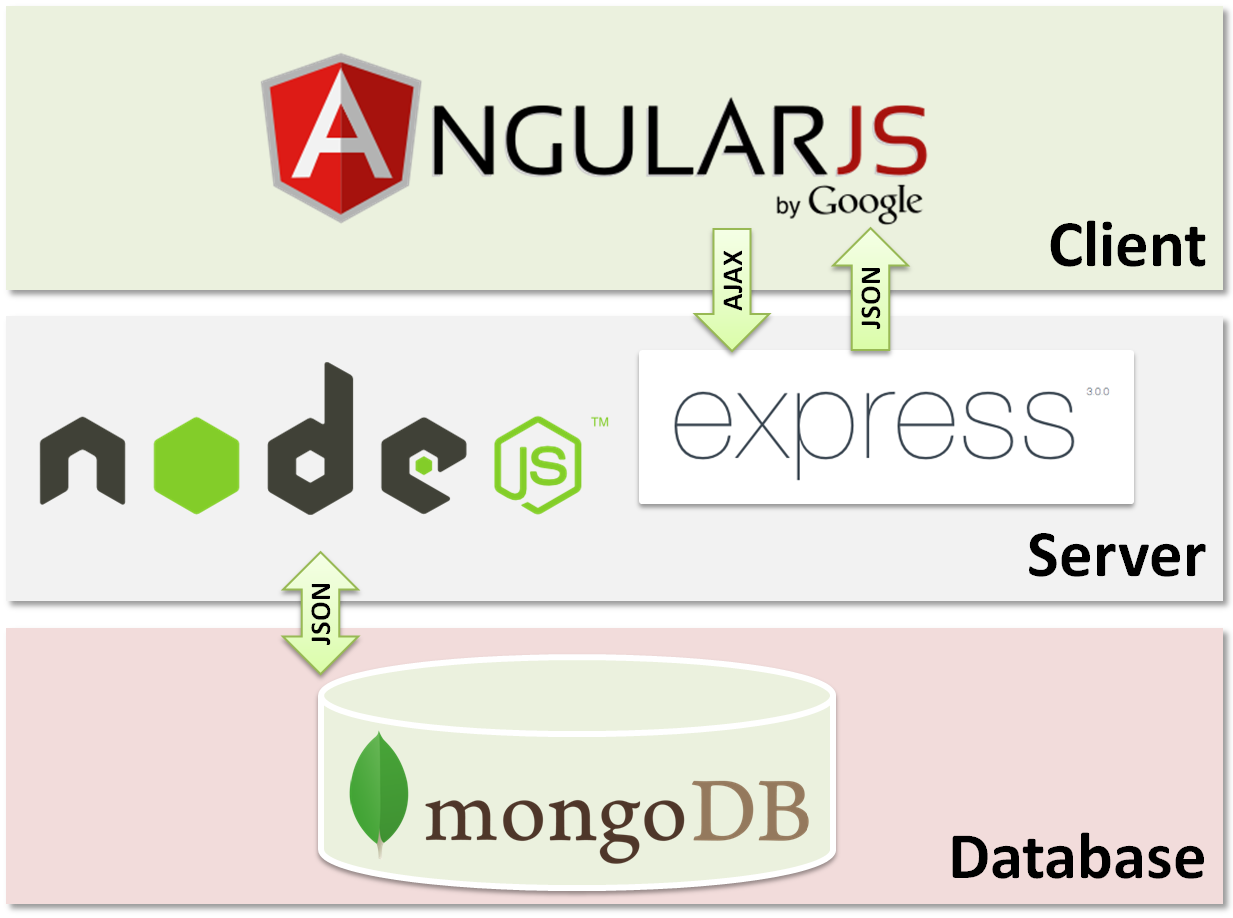
\includegraphics[scale=0.5]{resources/mean_diagram.png}
\end{center}
\caption{\label{figcaption} A high-level visualization of how the different MEAN components interact}
\end{figure}

\newpage

\appendix{B}{Case Study of Schema Migration at Ten Thousand Coffees}
blah blah

\newpage

\end{document}
